\documentclass[12pt]{extarticle}
\usepackage{geometry}
\geometry{
a4paper,
total={170mm,257mm},
left=20mm,
top=20mm,
headheight=12pt
}

\usepackage[parfill]{parskip} % Activate to begin paragraphs with an empty line rather than an indent
\usepackage{graphicx} % Use pdf, png, jpg, or eps§ with pdflatex; use eps in DVI mode
% TeX will automatically convert eps --> pdf in pdflatex
\graphicspath{ {./Figures/} }
\usepackage{subcaption}
\usepackage{float}

\usepackage{amssymb,amsmath,amsthm}
\usepackage{commath}
\usepackage{longtable}
\usepackage[hyphens]{url}
\usepackage[dvipsnames]{xcolor}
\usepackage[unicode=true,colorlinks=true,urlcolor=CadetBlue,citecolor=black,linkcolor=black]{hyperref}
\PassOptionsToPackage{hyphens}{url} % url is loaded by hyperref
\usepackage{authblk}
      
%SetFonts
% newtxtext+newtxmath
\usepackage{newtxtext} %loads helv for ss, txtt for tt
\usepackage{amsmath}
\usepackage[bigdelims]{newtxmath}
\usepackage[T1]{fontenc}
\usepackage{textcomp}
%SetFonts

% less space before sections 
% \@startsection {NAME}{LEVEL}{INDENT}{BEFORESKIP}{AFTERSKIP}{STYLE} 
%            optional * [ALTHEADING]{HEADING} 
\makeatletter
 \renewcommand\section{\@startsection {section}{1}{\z@}%
     {-2.5ex \@plus -1ex \@minus -.2ex}%
     {1.3ex \@plus.2ex}%
    {\Large\bfseries}}
    
% Species names
%% Meta-Command for defining new species macros
\usepackage{xspace}

\newcommand{\species}[3]{%
  \newcommand{#1}{\gdef#1{\textit{#3}\xspace}\textit{#2}\xspace}}
  
\species{\yeast}{Saccharomyces cerevisiae}{S.~cerevisiae}
\species{\calbicans}{Candida albicans}{C.~albicans}
\species{\cneoformans}{Cryptococcus neoformans}{C.~neoformans}

% Yoav & Lee commands
\newcommand*{\tr}{^\intercal}
\let\vec\mathbf
\newcommand{\matrx}[1]{{\left[ \stackrel{}{#1}\right]}}
\newcommand{\diag}[1]{\mbox{diag}\matrx{#1}}
\newcommand{\goesto}{\rightarrow}
\newcommand{\dspfrac}[2]{\frac{\displaystyle #1}{\displaystyle #2} }
\newtheorem{theorem}{Theorem}
\newtheorem{corollary}{Corollary}
\newtheorem{lemma}{Lemma}
\newtheorem{remark}{Remark}
\newtheorem{result}{Result}
\renewcommand\qedsymbol{} % no square at end of proof
\newcommand{\cl}{\mathbf{L}}
\newcommand{\cj}{\mathbf{J}}
\newcommand{\ci}{I}

% NatBib
\usepackage[round,colon]{natbib}

% Title page
\title{Cultural Transmission Can Explain the Evolution of Cooperative Behavior}

% Authors
\renewcommand\Affilfont{\small}

\author[1]{Dor Cohen}
\author[2]{Ohad Lewin-Epstein}
\author[3]{Marcus W. Feldman}
\author[a,*]{Yoav Ram}

\affil[1]{School of Computer Sciences, IDC Herzliya, Herzliya, Israel}
\affil[2]{School of Plant Sciences and Food Security, Tel Aviv University, Tel Aviv, Israel}
\affil[3]{Department of Biology, Stanford University, Stanford, CA}
\affil[*]{Corresponding author: yoav@yoavram.com}

\date{\today}

\begin{document}
\maketitle

% Abstract
%\begin{abstract}
%\end{abstract}

\pagebreak

% Introduction
\section*{Introduction}
Cooperative behavior can harm the individual's fitness and increase the fitness of its competitor~\citep{axelrod1981evolution}.
Yet, cooperative behavior occurs in many non-human animals~\citep{dugatkin1997cooperation}, for example rats~\citep{rice1962altruism} and birds~\citep{krams2008experimental}.
Therefore, the evolution of cooperative behavior is an important open question in evolutionary biology.
\\
Cultural evolution is an evolutionary theory of social change.
Culture has significant impact on the behavior of humans~\citep{ihara2004cultural,jeong2018bronze} as well as non-human animals~\citep{bonner2018evolution}.
Under the view of cultural evolution, an individual can acquire its behavior from another individual in its social group through learning or other modes of cultural transmission \citep{richerson2008not}.
Here we attempt to determine to what extent cultural transmission can explain the evolution of cooperative behavior.

% subsection
\subsection*{Theories for evolution of cooperation}
Three major theories have been proposed to explain the evolution of cooperative behavior.

\paragraph{Kin selection theory} suggests that natural selection can favor cooperative behavior between kin. The importance of relatedness to the evolution of cooperation and altruism was shown by~\citet{hamilton1964genetical}. According to Hamilton, kin selection causes allele to increase in frequency when the the reproductive cost to the actor, $c$, is less than the benefit to the recipient, $b$, times the genetic relatedness between the recipient and the actor, $r$.
This is also known as Hamilton's Rule:

\begin{equation} \label{eq:hamilton_rule}
c < b \cdot r.
\end{equation}

There is an ongoing debate about to what extent kin selection explains evolution of cooperation and altruism.
It has been suggested that kin selection to explain the cooperative behavior of eusocial insects like the honey bee.
The most significant argument against kin selection is that cooperation can evolve with zero relatedness~\citep{wilson2005kin}. This makes Hamilton's rule incomplete according to \citet{wilson2005kin}. \citet{foster2006kin} reject this claim. They argue that altruism without relatedness can not evolve. They refer us to Hamilton who claimed that relatedness can arise without recent common ancestry. 
\citet{wilson2005kin} also criticizes kin selection on the grounds that environmental or ecological factors probably be more important than relatedness in determining social actions. On the other hand, \citet{foster2006kin} argue that kin selection does not ignore ecology. Hamilton's rule shows
that environmental factors causing a high benefit-to-cost ratio will favor cooperation.

\paragraph{Reciprocity} suggests repeating interactions or individual recognition as key factors for explaining the evolution of cooperation. In \emph{direct reciprocity} there are a repeated encounters between the same two individuals. In every encounter, each player has a choice between cooperation and defection. If I cooperate now, you may cooperate later. Hence, it may pay off to cooperate.
This game-theoretic framework is known as the repeated Prisoner's Dilemma. 
%A well known strategy to play this game is called  'tit-for-tat'. This strategy always starts with a cooperation, then it does whatever the other player has done in the previous round: a cooperation for a cooperation, a defection for a defection. There a unlimited number of possible strategies to play this game. However, 
Direct reciprocity can only lead to the evolution of cooperation if the cost is less than the benefit $b$ times the probability for another encounter between the same two individuals, $w$, 

\begin{equation} \label{eq:reciprocity}
c < b \cdot w.
\end{equation}

Direct reciprocity assumes that both players are in a position to cooperate. Direct reciprocity can not explain cooperation in asymmetric interactions. In humans, such interactions happen often, for example humans often donate money. 

\paragraph{Indirect reciprocity} has been suggested to explain this behavior.
\citet{nowak2006five} claims that direct reciprocity is like a barter economy based on the immediate exchange of goods, while indirect reciprocity resembles the invention of money. The money that "fuels the engines" of indirect reciprocity is reputation. 
However, Reciprocity assume repeating interactions and therefore, has difficulty explaining evolution of cooperation if the no repeating interactions occurs. 

\paragraph{Group selection theory} posits that cooperation is favored because of the advantage to the whole group, if selection acts at the group level in addition to the individual level. A common model for group selection work as is: the population is divided into groups. In each groups there are cooperators, which help to other group members and defectors which do not help.  % TODO add reference
Individuals reproduce proportional to their fitness. Offspring are added to the same group.
If a group reaches a certain size it can split to two groups. A group that grow faster will split more often.
Groups of cooperators are growing faster than group of defectors.
Therefore, cooperation can evolve in this model when the cost $c$ is less than the benefit $b$ times the ratio between the  the number of groups $m$ and the sum of $m$ and the maximum group size $n$,

\begin{equation} \label{eq:groupselection}
c < b \cdot \frac{m}{m+n} .
\end{equation}

Group selection was criticized by biologists advocate gene-centered view of evolution. Group selection has been criticized due to the fact that the trait like cooperation evolves in the total population. According to natural selection, if cooperation took over the population it must have better fitness. However, in group selection the fitness of cooperator in the individual level is lower. The fact that a trait with a lower fitness took over the population is a contradiction. \citet{eldakar2011eight} reject this argument. They believe that this argument is a tautology and does not qualify as an argument against group selection. The distinction between individual and group selection requires a comparison of fitness differentials within and among groups in a multi group population. When a trait is evolve by group selection, despite the fact that it has lower fitness within the group, it has a better fit, all thing considered. 

\paragraph{}
All the above theories assume that cooperation is genetically determined. This raises the question, is it possible that cooperation is determined by non-genetic factors?
Recent work by \citet{lewin2017microbes} sheds some light on this question. 
\citet{lewin2017microbes} have hypothesised that microbes that manipulate their hosts to act altruistically can be favored by selection, and may play a role in the widespread occurrence of cooperative behavior. Indeed, it has been shown that microbes can mediate behavioral changes in their hosts~\citep{poulin2010parasite,dobson1988population}. Therefore, natural selection on microbes may favor manipulation of the host so that it cooperates with others. Microbes can be transmitted \emph{horizontally} from one host to another during host interactions. Following horizontal transfer, the recipient host may carry microbes that are closely related to the microbes of the donor host, even when the two hosts are (genetically) unrelated~\citep{lewin2017microbes}. Microbes can also transfer vertically, from parent to offspring. % yr: cite 10.1126/science.aat7164
As a result, a microbe that induces its host to cooperate with another host and thereby increases the other host fitness will  increase the vertical transmission of the microbes of the receiving individual. Kin selection among microbes could therefore favor microbes that induce cooperative behavior in their hosts, thereby increasing the transmission of their microbial kin.
%\\While the hypothesis that microbes could manipulate their hosts to act altruistically is mathematically feasible~\citep{lewin2017microbes}, there are still no empirical evidence of whether microbes indeed mediate altruistic behavior of their hosts.

% subsection
\subsection*{Cultural evolution of cooperation}
\citet{lewin2017microbes} have demonstrated that \emph{non-vertical transmission} can help to explain the evolution of cooperative behavior. 
Non-vertical transmission could be either a horizontal or oblique. Horizontal transmission occurs between individuals from the same generation. Oblique transmission occurs from an adult to an offspring. 
Evolution under either of these transmission models is can be be more rapid than under pure vertical transmission~\citep{ram2018evolution}. % (yr: not sure that this is a good reference)

Here we suggest a model in which behavioral changes are mediated by cultural transmission that can occur during social interaction. For example, if an individual interacts with a cooperative individual, it might learn that cooperation is a positive behavior and will cooperate in the future. Surprisingly, some of the analysis made by \citet{lewin2017microbes} can be applied to cultural transmission, because cultural transmission is mathematically akin to transmission of infectious diseases~\citep{cavalli1981cultural}.

Here, we hypothesize that non-vertical cultural transmission can explain the evolution of cooperation. We are develop cultural evolution models that include both vertical and non-vertical transmission of cooperation and investigate these models using both mathematical analysis and simulations. 

% Models and Methods
\section*{Models and Methods}

First, we focus on the evolution of cooperation in a fully mixed population where cooperation is modeled using the prisoner's dilemma. % yr: add ref

Consider a very large population whose members are characterized by their phenotype $\phi$, which can be of two types, $\phi=A$ for cooperators or $\phi=B$ for defectors, with corresponding fitness values $w_A$ and $w_B$, which depend on the frequency of the phenotypes (see below).
An offspring inherits its phenotype from its parent via vertical transmission with probability $v$ or from a random individual in the parental population via oblique transmission with probability $(1-v)$. 
Following~\citet{ram2018evolution}, given that the parent phenotype is $\phi$ and assuming uni-parental inheritance, % yr: cite Zefferman Behav Ecol 2016
the conditional probability that the phenotype $\phi'$ of the offspring is $A$ is 

\begin{equation} \label{eq:vertical_oblique_transmission}
P(\phi'=A \mid \phi) = \begin{cases}
v + (1-v)p, & \text{if } \phi=A \\
(1-v)p, & \text{if } \phi=B
\end{cases},
\end{equation}
where $p=P(\phi=A)$ is the frequency of $A$ among all adults in the parental generation.  

Not all adults become parents due to natural selection, and we denote the frequency of phenotype $A$ among parents with $\tilde{p}$.
Therefore, the frequency $\hat{p}$ of  phenotype $A$ among juveniles (after selection and vertical and oblique transmission) is

\begin{equation}\label{eq:horizontal}
\begin{aligned}
\hat{p}
& = \tilde{p} [v + (1-v)p] + (1-\tilde{p}) [(1-v)p] \\
& = v \tilde{p} + (1-v) p.
\end{aligned}
\end{equation}

Individuals interact in a social interaction modeled as a prisoner's dilemma.
Specifically, individuals interact in pairs, cooperators pay a fitness cost $0<c<1$, and their partner gains a fitness benefit $b$, where we assume $b>c$. The following payoff matrix shows the fitness of an individual with phenotype $\phi_1$ when interacting with a partner with phenotype $\phi_2$ ($b>c>0$):

\begin{table}[h]\label{table:prisoner_payoff}
\centering
\begin{tabular}{lll}
           & $\phi_2=A$ & $\phi_2=B$ \\
$\phi_1=A$ & $b-c$      & $-c$       \\
$\phi_1=B$ & $b$        & $0$       
\end{tabular}
\end{table}

Social interactions occur randomly.
So, two individuals with phenotype $A$ interact with probability $\hat{p}^2$, two individuals with phenotype $B$ interact with probability $(1-\hat{p})^2$, and two individuals with different phenotypes interact with probability $2\hat{p}(1-\hat{p})$. 

%Therefore, the fitness values of the two phenotypes, $w_A$ and $w_B$ are
%
%\begin{equation}\label{eq:fitness}
%\begin{aligned}
%w_A(\hat{p}) & = \hat{p}(1+b-c) + (1-\hat{p})(1-c) = 1 - c + \hat{p} b \\
%w_B(\hat{p}) & = \hat{p}(1+b) + (1-\hat{p}) = 1 + \hat{p} b,
%\end{aligned}
%\end{equation}
%and the population mean fitness is therefore
%$\bar{w} = \hat{p} w_A + (1-\hat{p}) w_B = 1 + \hat{p}(b-c)$.

Horizontal cultural transmission occurs between peers. 
It may occur between social partners with probability $\alpha$, or between a random pair with probability $1-\alpha$ (see~\textbf{\autoref{fig:horizontal}}).
Horizontal transmission is not always successful, as one peer may reject the other's phenotype. The probability for successful transmission of phenotypes $A$ and $B$ are $T_A$ and $T_B$, respectively.\\
\autoref{table:1} contains the probability of first interactor to be A following interaction by interaction type.
Therefore, the frequency $p'$ of phenotype $A$ among adults in the next generation, after horizontal transmission, is 
\begin{equation}\label{eq:nextgen_adults}
\begin{aligned}
p'
& = \hat{p}^2 [\alpha + (1-\alpha)(\hat{p} + (1-\hat{p})(1-T_B))] \\
& + \hat{p}(1-\hat{p}) [\alpha(1-T_B) + (1-\alpha)(\hat{p} + (1-\hat{p})(1-T_B))] \\
& + (1-\hat{p})\hat{p} [\alpha T_A + (1-\alpha) \hat{p} T_A ] \\
& + (1-\hat{p})^2 [(1-\alpha) \hat{p} T_A] \;,
\end{aligned}
\end{equation}
which can be simplified into
\begin{equation}\label{eq:nextgen_adults_slimpify}
p' = \hat{p}^2(T_B-T_A) + \hat{p}(1+T_A-T_B) .
\end{equation}

The frequency of $A$ among parents follows a similar dynamic, but also includes the effect of natural selection, and is therefore
\begin{equation}\label{eq:nextgen_parents}
\begin{aligned}
\bar{w} \tilde{p}'
& = \hat{p}^2 (1+b-c) [\alpha + (1-\alpha)(\hat{p} + (1-\hat{p})(1-T_B))] \\
& + \hat{p}(1-\hat{p}) (1-c) [\alpha(1-T_B) + (1-\alpha)(\hat{p} + (1-\hat{p})(1-T_B))] \\
& + (1-\hat{p})\hat{p} (1+b) [\alpha T_A + (1-\alpha) \hat{p} T_A ] \\
& + (1-\hat{p})^2 [(1-\alpha) \hat{p} T_A] \;,
\end{aligned}
\end{equation}
where fitness values are taken from \autoref{table:1}, and 
\begin{equation} \label{eq:mean_fitness}
\bar{w} = \hat{p} w_A + (1-\hat{p}) w_B = 1 + \hat{p}(b-c)
\end{equation}
is the population mean fitness.
Eq~\ref{eq:nextgen_parents} can be slimpified to
\begin{equation}\label{eq:nextgen_parents_simplified}
\begin{aligned}
\bar{w} \tilde{p}'
& = \hat{p}^2 (1+b-c) \big(1-(1-\hat{p})(1-\alpha)T_B)\big) \\
& + \hat{p}(1-\hat{p}) (1-c) \big(\hat{p}(1-\alpha)T_B+1-T_B\big) \\
& + (1-\hat{p})\hat{p} (1+b) \big(\hat{p}(1-\alpha) + \alpha\big) T_A \\
& + (1-\hat{p})^2 \hat{p} (1-\alpha) T_A \;.
\end{aligned}
\end{equation}

\begin{table}[H]
\begin{tabular}{|c|c|c|c|c|}
\hline
\textbf{Interaction Type} & \textbf{Frequency}    & \textbf{Fitness}      & \multicolumn{2}{c|}{\textbf{\begin{tabular}[c]{@{}c@{}}Probability of first interactor\\  to be A following interaction\end{tabular}}}                                                                                                     \\ \hline
\multicolumn{1}{|l|}{}    & \multicolumn{1}{l|}{} & \multicolumn{1}{l|}{} & \textbf{\begin{tabular}[c]{@{}c@{}}Horizontal transmission\\  from partner, \\ probability $\alpha$\end{tabular}} & \textbf{\begin{tabular}[c]{@{}c@{}}Horizontal transmission \\ from population, \\ probability $1-\alpha$\end{tabular}} \\ \hline
$AxA$                     & $\hat{p}^2$           & $1+b-c$               & $1$                                                                                                               & $\hat{p}+(1-\hat{p})(1-T_B)$                                                                                           \\ \hline
$AxB$                     & $\hat{p}(1-\hat{p})$  & $1-c$                 & $1-T_B$                                                                                                           & $\hat{p}+(1-\hat{p})(1-T_B)$                                                                                           \\ \hline
$BxA$                     & $\hat{p}(1-\hat{p})$  & $1+b$                 & $T_A$                                                                                                             & $\hat{p}T_A$                                                                                                           \\ \hline
$BxB$                     & $(1-\hat{p})^2$       & $1$                   & $0$                                                                                                               & $\hat{p}T_A$                                                                                                           \\ \hline
\end{tabular}
\caption{Fitness and probabilityof first interactor to be A following interaction by interaction type}
\label{table:1}
\end{table}

\begin{figure}[b]
  \centering
  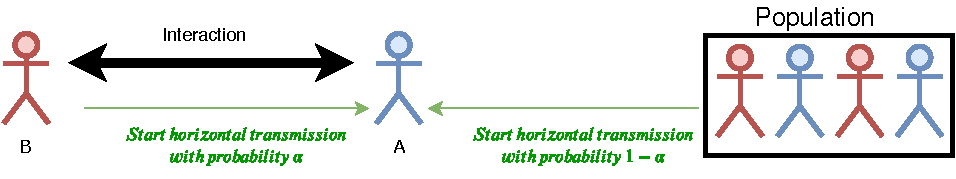
\includegraphics[scale=1]{figure1.pdf}
  \caption{\textbf{Cultural horizontal transmission.} Transmission occurs between interaction partners with probability $\alpha$ (left) or between two random peers with probability $1-\alpha$.}
  \label{fig:horizontal}
\end{figure}

% Results
\section*{Results}

We start by inspecting specific cases, for which we can derive general results. 
Afterwards, we use numerical simulation to analyze more complex cases.

%%%%%%%%%%%%%%%%%%%%%%%%%%%%%%%%%%%%%%%%%%%%%%%%
\subsection*{Without Oblique Transmission}

With only vertical and horizontal transmission, i.e. $v=1$, eq.~\ref{eq:horizontal} becomes
$\hat{p} =  \tilde{p}$,
and eq.~\ref{eq:nextgen_parents_simplified} for the change in frequency $p'$ of phenotype $A$ among parents can be written as

\begin{equation} 
\begin{split}\label{eq:nextgen_parents_vertical_only}
\bar{w} \tilde{p}' 
& = \tilde{p}^2 (1+b-c) [1 - (1-\tilde{p}) (1-\alpha) T_B] \\
& + \tilde{p}(1-\tilde{p}) (1-c) [\tilde{p} (1-\alpha) T_B + 1 - T_B] \\
& + \tilde{p}(1-\tilde{p}) (1+b) [\tilde{p} (1-\alpha) + \alpha] T_A \\
& + (1-\tilde{p})^2 \tilde{p} (1-\alpha) T_A
\end{split}
\end{equation}

We find the following result and corollaries.

\textbf{Result 1: Vertical and horizontal transmission of cooperation.}
If 
\begin{equation} \label{eq:unequal_transmission}
c \cdot (1-T_B) < b \cdot  \alpha T_A  + (T_A - T_B) [1 + b\tilde{p}(1-\alpha)]
\end{equation}
then $\tilde{p}' > \tilde{p}$, and the frequency of the cooperator phenotype $A$ among parents increases every generation.

\textbf{Corollary 1.1: Symmetric horizontal transmission.}
If $T=T_A=T_B$, then
\begin{equation}
\label{eq:equal_transmission}
c < b \cdot \frac{\alpha T}{1-T},
\end{equation}
which can be seen as a cultural version of \emph{Hamilton's rule} (eq.~\ref{eq:hamilton_rule}), where $r_H=\alpha T/(1-T)$ can be thought of as \emph{horizontal relatedness}.
Therefore, if the cost $c$ is less than the benefit $b$ times the horizontal relatedness $r_H$, then cooperation will take over of the population (see~\textbf{\autoref{fig:results_a}}).

\textbf{Corollary 1.2: Complete correlation between transmission and cooperation.}
	
In this case $\alpha=1$, and horizontal transmission can only occur as a result of cooperative interactions.
Therefore, eq.~\ref{eq:unequal_transmission}, which determines the conditions for evolution of cooperation, becomes
\begin{equation}\label{eq:horizontal_transmission_only_after_interaction}
c \cdot (1-T_B) < b \cdot T_A + (T_A - T_B).
\end{equation}
This is equivalent to a result by~\citet[eq.~1]{lewin2017microbes}.

Eq.~\ref{eq:horizontal_transmission_only_after_interaction} can be written as
\begin{equation} \label{eq:horizontal_transmission_only_after_interaction2}
1 - (1-T_B)(1-c) < T_A \cdot (1+b) ,
\end{equation}
which provides an interesting interpretation for the success of cooperation. 
Consider an interaction between two individuals: a cooperator and a defector.
$(1-T_B)(1-c)$ is the probability that the cooperator remains cooperative and also reproduces. 
Therefore, $1 - (1-T_B)(1-c)$ is the probability that either the cooperator becomes a defector, \emph{or} that it fails to reproduce.
This is the effective cost for cooperation from this interaction.
$T_A\cdot(1+b)$ is the probability that the defector becomes cooperative and reproduces.
This is the effective benefit for cooperation from this interaction.
So, eq.~\ref{eq:horizontal_transmission_only_after_interaction2} means that cooperation can evolve if effective cost is less than the effective benefit.

\textbf{Corollary 1.3: No correlation between transmission and cooperation.}

In this case $\alpha=0$, and horizontal transmission is entirely independent from cooperative interactions.  
Then, eq.~\ref{eq:unequal_transmission} becomes
\begin{equation} \label{eq:horizontal_transmission_from_population}
c\cdot(1-T_B) < b \cdot \tilde{p} \;(T_A-T_B) + (T_A-T_B). 
\end{equation}

Therefore, because all the parameters are all positive, cooperation cannot take over the population (and furthermore will become extinct) if cooperators doesn't have a horizontal transmission bias, i.e. if $T_A\leq T_B$.
When such a bias does exist, $T_A > T_B$, then cooperation will evolve if $\tilde{p} > \tilde{p}^{*}$, where (see also ~\textbf{\autoref{fig:results_b}})
\begin{equation} 
\begin{split} \label{eq:horizontal_transmission_from_population_equilibrium}
\tilde{p}^{*} & = \frac{c}{b} \cdot \frac{1-T_B}{T_A-T_B} - \frac{1}{b}.
\end{split}
\end{equation}
A sufficient condition for evolution of cooperation is that $\tilde{p}^{*} < 0$, which occurs if
\begin{equation} \label{eq:sufficient_horizontal_transmission_from_population}
c < \frac{T_A-T_B}{1-T_B} .  
\end{equation}


%%%%%%%%%%%%%%%%%%%%%%%%%%%%%%%%%%%%%%%%%%%%%%%%
\subsection*{Without Vertical Transmission}

With only oblique and horizontal transmission, i.e. $v = 0$, eq.~\ref{eq:horizontal} becomes $\hat{p}=p$ and eq.~\ref{eq:nextgen_adults_slimpify} becomes % TODO check this, I changed the ref from nextgen_parents_simplified to nextgen_adults_slimpify
\begin{equation}  \label{eq:nextgen_parents_oblique_only}
p' = p^2 (T_B-T_A) + p (1+T_A-T_B) .
\end{equation}

We find the following results.

\textbf{Result 2: Oblique and horizontal transmission of cooperation.} The frequency of phenotype $A$ among adults increases if $p'>p$.
Using eq.~\ref{eq:nextgen_parents_oblique_only}, we find that $p'>p$ occurs when
\begin{equation} \label{eq:oblique_only_result}
T_A > T_B . 
\end{equation}
Therefore, cooperation will evolve if the cooperator phenotype has a horizontal transmission bias (see~\textbf{\autoref{fig:results_c}}).

%%%%%%%%%%%%%%%%%%%%%%%%%%%%%%%%%%%%%%%%%%%%%%%%
\subsection*{With Vertical and Oblique Transmission}

In this case $0<v<1$, and the equation system is more complex than before.
Therefore, we focus on local rather than global stability, which was the case so far.\\
To proceed, we note that 
eq.~\ref{eq:horizontal} can give $\hat{p}'$ as a function of both $p'$ and $\tilde{p}'$,
eq.~\ref{eq:nextgen_adults_slimpify} gives $p'$ as a function of $\hat{p}$, and 
eq.~\ref{eq:nextgen_parents_simplified} gives $\tilde{p}'$ as a function of $\hat{p}$. 
Combining these equations, we find an equation for $\hat{p}'$ as a function of $\hat{p}$.
We then determine the equilibria of this equation, that is, solutions for $\hat{p}' = \hat{p}$, and their stability.

\textbf{Result 3: Oblique and vertical transmission with symmetric horizontal transmission.}

For simplicity, we start with the assumption that $T_A = T_B = T$. We have
\begin{equation} \label{eq:equal_horizontal_transmission}
% DOR: I checked again, substituting eq 7 and 9 to eq 5: you have to divide the RHS by wbar.
  %\hat{p}' - \hat{p} = 
  %\hat{p} ^2(-\alpha bvT + cv(1-T)) + \hat{p} (\alpha bvT -cv(1-T)) = 
  \bar{w}(\hat{p}' - \hat{p}) = 
  f(\hat{p}) = \hat{p}(1-\hat{p})(\alpha bvT - cv(1-T)) % shorter version
\end{equation}

We are looking for the equilibrium $\hat{p}^*$ which occurs when $f(\hat{p}^*)=0$, or $\hat{p}' = \hat{p}$.
It is easy to verify that fixation of either phenotype is an equilibrium, that is,
\begin{equation} \label{eq:result2.1}
  \hat{p}^*_0 =  0, \, \hat{p}^*_1 = 1 .
\end{equation}

Is fixation of cooperation, $\hat{p}^*_1=1$, locally stable?. 
An equilibrium point $\hat{p}^*$ is locally stable when the derivative of $f(\hat{p})$ at $p^*$ is negative, $f'(\hat{p}^*)<0$. 
This derivative is
\begin{equation} \label{eq:derivative_of_phattag-phat}
	f'(\hat{p}) \mid_{\hat{p}=1} = 
% 2\cdot\hat{p} (-\alpha bvT + cv(1-T)) + (\alpha bvT -cv(1-T)).
	(1- 2\hat{p}) (\alpha bvT - cv(1-T)) \mid_{\hat{p}=1} = 
	-\alpha bvT + cv(1-T)).
\end{equation}
Therefore, fixation of cooperation is locally stable when
\begin{equation} \label{eq:oblique_and_vertic_result2}
  %\frac{b}{c}>\frac{1-T}{\alpha T}
	c < b \cdot \frac{\alpha T}{1-T},
\end{equation}
which is the same condition we found in Corollary 1.1, Eq.~\ref{eq:equal_transmission}.

\textbf{Result 4: Oblique and vertical transmission of cooperation with asymmetric horizontal transmission.}

We now study the general case where $T_A \neq T_B$. We have
\begin{equation} \label{eq:general_case_polynomial}
  f(\hat{p}) = \bar{w}(\hat{p}'-\hat{p}) =
  \beta_1 \hat{p}^3 + \beta_2 \hat{p}^2 + \beta_3 \hat{p},
\end{equation}
where 
\begin{equation} \label{eq:polynomial_coefficients}
\begin{aligned}
\beta_1 &= \big[c(1-v) - b (1-\alpha v)\big] (T_A-T_B) \\
%\beta_2 &= -[c(1-v) - b(1-\alpha v) +  1](T_A-T_B)-\alpha bv T_A + cv(1-T_B) \\
\beta_2 &= -\beta_1 -\beta_3  \\
\beta_3 &= \alpha bvT_A - cv(1-T_B) + (T_A-T_B) .
\end{aligned}
\end{equation}
Since $f(\hat{p})$ is a cubic polynomial, three equilibria exist.
We already know that $\hat{p}^*_0 = 0 $ and $\hat{p}^*_1 = 1$ are equilibria.
The third equilibrium $\hat{p}^*_2$ can be found by solving $f(\hat{p})/\big[\hat{p}(1-\hat{p})\big] = \beta_3 -\beta_1 \hat{p} = 0$:
\begin{equation} \label{eq:oblique_and_vertic_result}
  \hat{p}^*_2 =  
  \frac{\beta_3}{\beta_1}.
  %\frac{\alpha bvT_A - cv(1-T_B) + (T_A-T_B)}
  %     {\big(c(1-v) -b (1-\alpha v)\big) (T_A-T_B)} .
\end{equation}
To determine when $\hat{p}^*_2$ is a legitimate equilibrium (i.e. $0<\hat{p}^*_2<1$), we first focus on the left inequality, $0<\hat{p}^*_2$, and
%To do that we find the derivative  of $f(\hat{p})$,
%\begin{equation} \label{eq:derivative_of_phattag-phat2}
%  f'(\hat{p}) = 3\beta_1 \hat{p}^2 + 2\beta_2\hat{p}^2 + \beta_3
% \end{equation}
assume that $T_A>T_B$. In this case,
\begin{equation} \label{eq:beta1}
  \begin{split}
   \beta_1 & = [c(1-v) - b (1-\alpha v)] (T_A-T_B) \\
   &< [c(1-\alpha v) - b(1-\alpha v)] (T_A-T_B) \\
   &= (1-\alpha v)(c-b)(T_A-T_B) < 0 ,
  \end{split}
 \end{equation}
since $T_A > T_B$, $c<b$, and $1>\alpha v$.
Therefore, when $\hat{p}$ goes to negative infinity, the cubic $f(\hat{p})$ goes to positive infinity.
So, a necessary condition for $\hat{p}^*_2>0$ is that $f'(0) = \beta_3 < 0$.
This condition also satisfies local stability of $\hat{p}^*_0=0$.
Hence, if $\hat{p}^*_2$ is legitimate, then extinction of cooperation is locally stable. 

We now focus on $\hat{p}^*_2<1$, still assuming $T_A>T_B$.
When $\hat{p}$ goes to positive infinity, the cubic $f(\hat{p})$ goes to negative infinity (Eq.~\ref{eq:beta1}).
So, a necessary condition for $\hat{p}^*_2<1$ is that $f'(1)=\beta_1 - \beta_3<0$.
This condition also satisfies local stability of $\hat{p}^*_1=1$.
Hence, if $\hat{p}^*_2$ is legitimate, then fixation of cooperation is also locally stable.
Moreover, since legitimacy of $\hat{p}^*_2$ implies local stability of both $\hat{p}^*_0$ and $\hat{p}^*_1$, we conclude that $\hat{p}^*_2$ is locally unstable.

If we assume instead that $T_A < T_B$, we reach the following results:

\textbf{Result 4}: if $T_A>T_B$ ($T_B>T_A$), then $\hat{p}^*_2$ is a legitimate locally unstable equilibrium when $\beta_1<\beta_3<0$ ($\beta_1>\beta_3>0$). In this case, both fixations are locally stable and $\hat{p}^*_2$ separates the domains of attraction.


\begin{figure}[H]
  \centering
  \begin{subfigure}{8cm}
    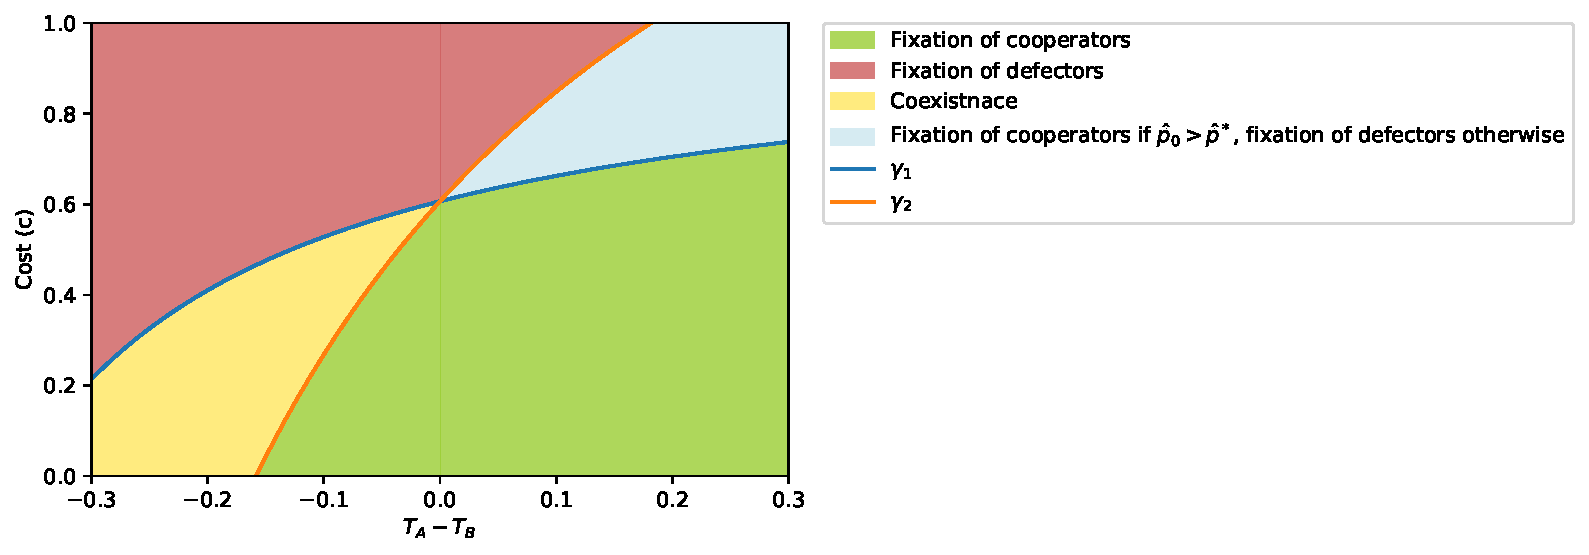
\includegraphics[scale=0.5]{figure2a.pdf}
    \caption{$v=1$, $T_A=T_B=T$, $\alpha \neq 0$}
    \label{fig:results_a}
  \end{subfigure}
  \begin{subfigure}{8cm}
    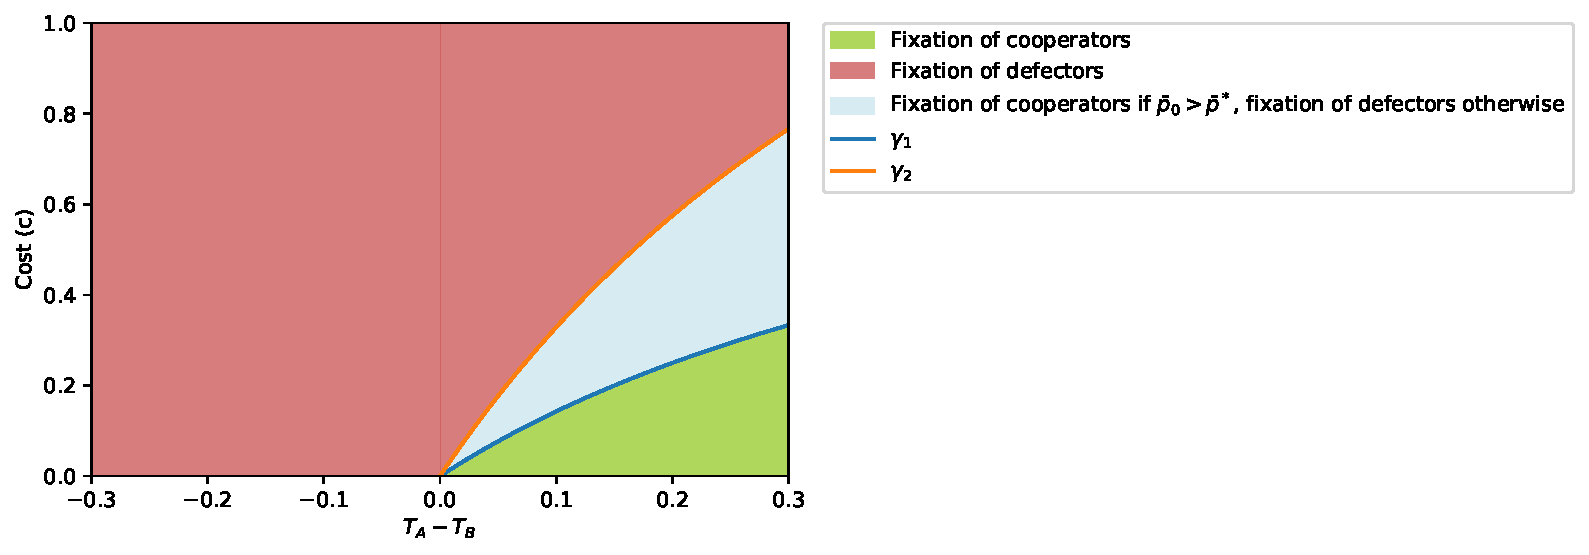
\includegraphics[scale=0.5]{figure2b.pdf}
    \caption{$v=1$, $\alpha = 0$}
    \label{fig:results_b}
  \end{subfigure}
  \begin{subfigure}{8cm}
    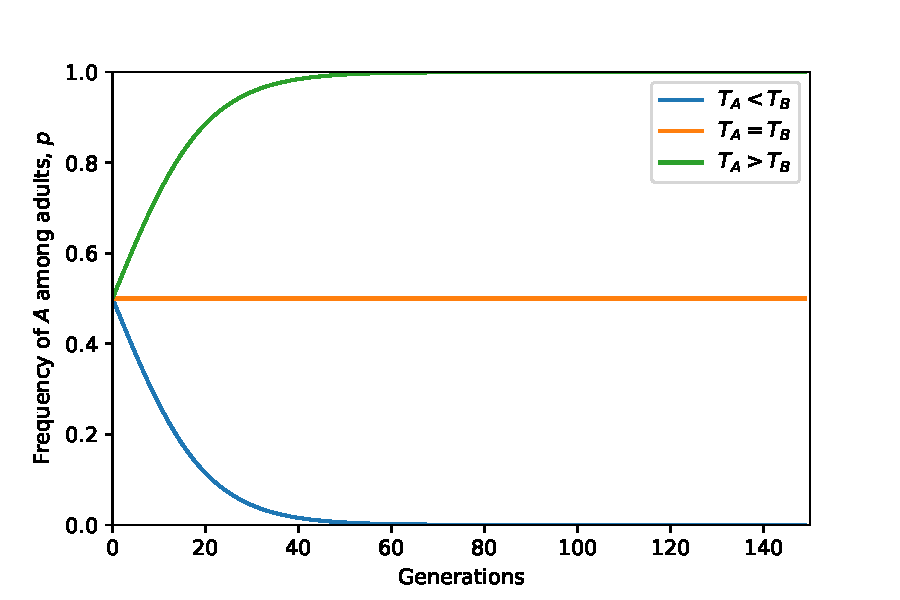
\includegraphics[scale=0.5]{figure2c.pdf}
    \caption{$v=0$}
    \label{fig:results_c}
  \end{subfigure}
  \label{fig:results}
  \caption{
  \textbf{Numerical results for cultural evolution of cooperation.}
  Shown are dynamics of \textbf{(a-b)} $\tilde{p}$, the frequency of parents with cooperative phenotype $A$; \textbf{(c)} $p'$, the frequency of adults with cooperative phenotype $A$.
  The figure demonstrates fixation of cooperation (green), extinction of cooperation (blue)m and stable co-existence of cooperators and defectors (orange). %TODO ic (c), the blue and green got mixed. 
  % TODO have all panels in one row.
  }
\end{figure}

% Discussion
\section*{Discussion}
We hypothesized that non-vertical transmission can explain the evolution of cooperation. We used a model with non-vertical transmissions and have found that if eq.~\ref{eq:unequal_transmission} is satisfied cooperation will take over the population in fully mixed population with prisoner's dilemma payoff. In addition, we found that when horizontal transmission cannot occur after interaction ($\alpha = 0$) cooperation will always become extinct. 
Our results improve our understating of cultural evolution of cooperation. Our model shows that cooperation can evolve even in a fully mixed population, where the population is non-structured, there are no repeating interactions and nor individual recognition.

%\pagebreak
% Acknowledgements
{\small
\section*{Acknowledgements}
We thank Lilach Hadany and Ayelet Shavit for discussions and comments.
This work was supported in part by
the Israel Science Foundation 552/19 (YR),
and Minerva Center for Lab Evolution (YR).
% TODO funding for other authors?
}

% Bibliography
\bibliographystyle{plainnat}
\bibliography{bib}

% Appendices
\newpage
\section*{Appendix A} % TODO fix equations references
In the section, we start with eq.~\ref{eq:nextgen_parents_vertical_only} and we want to investigate when $\tilde{p}< \tilde{p}'$. 
\begin{equation} 
\begin{split} \label{eq:horizontal_transmission_from_interaction_step0}
\bar{w}\tilde{p} < & \, \tilde{p}^2 (1+b-c) (1 - (1-\tilde{p}) (1-\alpha) T_B) \\
& + \tilde{p}(1-\tilde{p}) (1-c) (\tilde{p} (1-\alpha) T_B + 1 - T_B) \\
& + \tilde{p}(1-\tilde{p}) (1+b) (\tilde{p} (1-\alpha) + \alpha) T_A \\
& + (1-\tilde{p})^2 \tilde{p} (1-\alpha) T_A
\end{split}
\end{equation}
First divide by $\tilde{p}$, thus eq.~\ref{eq:horizontal_transmission_from_interaction_step0} becomes
\begin{equation} 
\begin{split} \label{eq:horizontal_transmission_from_interaction_step1}
  \bar{w} < & \, \tilde{p}(1+b-c) (1 - (1-\tilde{p}) (1-\alpha) T_B) \\
  & + (1-\tilde{p}) (1-c) (\tilde{p} (1-\alpha) T_B + 1 - T_B) \\
  & + (1-\tilde{p}) (1+b) (\tilde{p} (1-\alpha) + \alpha) T_A \\
  & + (1-\tilde{p})^2 (1-\alpha) T_A
\end{split}
\end{equation}
We know that the mean fitness $\bar{w} = 1 + \tilde{p}(b-c)$, thus eq.~\ref{eq:horizontal_transmission_from_interaction_step1} becomes
\begin{equation} 
\begin{split} \label{eq:horizontal_transmission_from_interaction_step2}
  1 + \tilde{p}(b-c) < & \, \tilde{p}(1+b-c) (1 - (1-\tilde{p}) (1-\alpha) T_B) \\
  & + (1-\tilde{p}) (1-c) (\tilde{p} (1-\alpha) T_B + 1 - T_B) \\
  & + (1-\tilde{p}) (1+b) (\tilde{p} (1-\alpha) + \alpha) T_A \\
  & + (1-\tilde{p})^2 (1-\alpha) T_A
\end{split}
\end{equation}
Eq.~\ref{eq:horizontal_transmission_from_interaction_step2} can be simplified into eq.~\ref{eq:unequal_transmission}.


\end{document}
